%! TeX program = xelatex

\documentclass[12pt, a4paper]{article}
\usepackage{cmap}
\usepackage[fontsize=12pt]{scrextend}
\usepackage[T2A]{fontenc}
\usepackage[utf8]{inputenc}
\usepackage[english,russian]{babel}
\usepackage{amsmath,amsfonts,amssymb,amsthm,mathtools}
\usepackage[left=20mm, top=20mm, right=20mm, bottom=20mm, nohead, footskip=1cm]{geometry}
\usepackage{multirow}
\usepackage{array}
\usepackage{multicol}
\usepackage{graphicx}
\usepackage{wrapfig}
\usepackage{indentfirst}
\usepackage{enumitem}

\usepackage{polyglossia}
\usepackage{titlesec}
\usepackage{sectsty}
\usepackage{setspace}
\usepackage{fontspec}
\defaultfontfeatures{Mapping=tex-text}

\usepackage{lipsum}
\usepackage{tocloft}
\usepackage[dvipsnames]{xcolor}

\usepackage{caption}
%\captionsetup{labelfont=it, textfont=it}
%\captionsetup[figure]{name=Схема}

\usepackage{hyperref}

\hypersetup{
    colorlinks=false,
    linktoc=all
}
\urlstyle{same}

\setmainlanguage{english}
\setotherlanguage{russian}
\setkeys{russian}{babelshorthands=true}
\setmainfont{Times New Roman}
\newfontfamily\cyrillicfont{Times New Roman}
\let\cyrillicfonttt\ttfamily
%\onehalfspacing

%\allsectionsfont{\centering}
\renewcommand{\cftsecleader}{\cftdotfill{\cftdotsep}}

%======================================SECTIONING=========================================
%\makeatletter
%\renewcommand*\l@section{\@dottedtocline{1}{1.5em}{2.3em}}
%\makeatother
%======================================SECTIONING=========================================

\pretolerance=6000
\tolerance=3000
\emergencystretch=4pt

\setlength\intextsep{10pt}

\graphicspath{{./visuals/}}
\setlength{\parskip}{0.3125cm}
\setlength{\parindent}{1.25cm}
\setlength{\columnsep}{1cm}
\author{Grigoryev Mikhail}
\title{Algs lab}

\begin{document}

\thispagestyle{empty}

\vspace{30mm}

\begin{center}
FEDERAL STATE AUTONOMOUS EDUCATIONAL INSTITUTION \\
OF HIGHER EDUCATION \\
ITMO UNIVERSITY

\vspace{40mm}

{\large \textbf{Report \\
on the practical task No. 4 \\
"Algorithms for unconstrained nonlinear optimization. Stochastic and metaheuristic algorithms"}}
\end{center}

\vspace{15mm}

\begin{flushright}
{\large Performed by \\
\textit{Mikhail Grigoryev (370852) \\
Semenova Valeria (370061) \\
Academic group J4133c \\}
Accepted by \\
Dr Petr Chunaev}
\end{flushright}

\vspace{80mm}

\begin{center}
St. Petersburg \\
2022
\end{center}

\newpage

\section*{Goal}
\addcontentsline{toc}{section}{Goal}

The use of stochastic and metaheuristic algorithms (Simulated Annealing, Differential Evolution, Particle Swarm Optimization) in the tasks of unconstrained nonlinear optimization and the experimental comparison of them with Nelder-Mead and Levenberg-Marquardt algorithms.

\section*{Formulation of the problem}
\addcontentsline{toc}{section}{Formulation of the problem}

\textbf{Task 1.} Generate the noisy data $(x_k, y_k)$, where $k = 0, \cdots, 1000$, according to the rule:
\[ y_k = \begin{cases}
	-100 + \delta_k,   & f(x_k) < -100             \\
	f(x_k) + \delta_k, & -100 \leq f(x_k) \leq 100 \\
	100 + \delta_k,    & f(x_k) > 100              \\
\end{cases} \]
\[ x_k = 0.003 \cdot k \qquad f(x) = \frac{1}{x^2 - 3x + 2} \]
where $\delta_k \sim N(0, 1)$ are values of a random variable with standard normal distribution. Approximate the data by the following rational function:
\[ F(x, a, b, c, d) = \frac{ax + b}{x^2 + cx + d} \]
by means of least squares through the numerical minimization (with precision $\varepsilon = 0.001$) of the following function:
\[ D(a, b, c, d) = \sum_{k=0}^{1000} \left( F(x_k, a, b, c, d) - y_k \right)^2 \]
To solve the minimization problem, use Nelder-Mead algorithm, Levenberg-Marquardt algorithm and at least two of the methods among Simulated Annealing, Differential Evolution and Particle Swarm Optimization (\textit{first two chosen}). If necessary, set the initial approximations and other parameters of the methods. At most 1000 iterations are allowed. Visualize the data and the approximants obtained in a plot separately for each for each type of \textbf{approximant} so that one can compare the results for the numerical methods used. Analyze the results obtained (in terms of number of iterations, precision, number of function evaluations, etc.).

\textbf{Task 2.} Choose at least 15 cities in the world having land transport connections between them. Calculate the distance matrix for them and then apply the Simulated Annealing method to solve the corresponding Travelling Salesman Problem. Visualize the results at the first and the last iteration. If necessary, use the city dataset from \newline
\url{https://people.sc.fsu.edu/~jburkardt/datasets/cities/cities.html}

\newpage

\section*{Brief theoretical part}
\addcontentsline{toc}{section}{Brief theoretical part}

Optimization methods are essentially methods of finding optimal (depens on the task) values of target functions. Often optimization is just minimizing a certain function.

The solution to the optimization (minimization) problem is finding:
\[ x^* \in Q: \quad f(x^*) = \min_{x\in Q} f(x) \def \arg \min_{x\in Q} f(x) \]
Finding the argument which corresponds to the function minimum will let us find the value of the function at its minimum.

In this practical work local minima will be found, $f(x)$ can be nonlinear and no additional constrictions on the argument will be applied. Hence the title, "unconstrained nonlinear optimization".

In addition to that, in this work stochastic and metaheuristic algorithms are used. Stochastic here refers to the algorithm to utilize random and probabilities to make predictions (non-deterministic). Metaheuristic algorithms are those that sacrifice completeness and precision for speed.

Algorithms used in this practical work:
\begin{enumerate}
	\item Simulated Annealing -- metaheuristic algorithm that lets current approximation take large steps with high probabilities at first (when the temperature is high). This helps to avoid globally unoptimal local minima. Implementation taken from Scipy.
	\item Differential Evolution -- metaheuristic algorithm that solves the optimization problem by maintaining a population of so-called agents (candidate solutions which create new agent using existing ones and keep the best one). The algorithm implementation was taken from Scipy.
\end{enumerate}

In the second task the path in the Travelling Salesman Problem was optimized by Simulated Annealing implemented from scratch. The path was optimized in a way that in each iteration cities were reconnected with a certain probability which depends on how optimal the new solution is and on the current temperature (the higher the temperature, the higher the probability of a jump).

\newpage

\section*{Results}
\addcontentsline{toc}{section}{Results}

\textbf{Task 1.} Noisy data was generated. Then, Nelder-Mead (task 2), Levenberg-Marquardt (task 3), Simulated Annealing and Differential Evolution methods of non-linear approximation were applied to the problem. The data obtained is presented in the table:
\begin{center}
\begin{tabular}{ccccccc}
\hline
alg/param                    & A & B & C & D & Iterations & Function calls \\ \hline
Nelder-Mead Search (Task 2)  & -1.0037 & 1.0042 & -2.0009 & 1.0009 & 399 & 665 \\
Levenberg-Marquardt (Task 3) & -1.0074 & 1.0078 & -2.0008 & 1.0008 & 123 & 123 \\
Differential Evolution       & -1.0070 & 1.0074 & -2.0009 & 1.0009 & 158 & 9700 \\
Simulated Annealing          & -1.0036 & 1.0041 & -2.0009 & 1.0009 & 4 & 1021 \\ \hline
\end{tabular}
\end{center}
All four methods gave close results. Interestingly, the approximations fit only data with $x < 1.5$. The resulting function predicted is:
\[ f(x) = \frac{1 - x}{x^2 - 2x + 1} \]
This may have happened due to the methods falling into local minima of the least squares loss function. Performance-wise, Levenberg-Marquardt is better than direct Nelder-Mead. Metaheuristic Simulated Annealing gave the best performance in terms of iterations. However, it required more than a thousand function calls. Differential Evolution proved to be the worst method in terms of iterations and function calls.

\begin{figure}[!h]
\centering
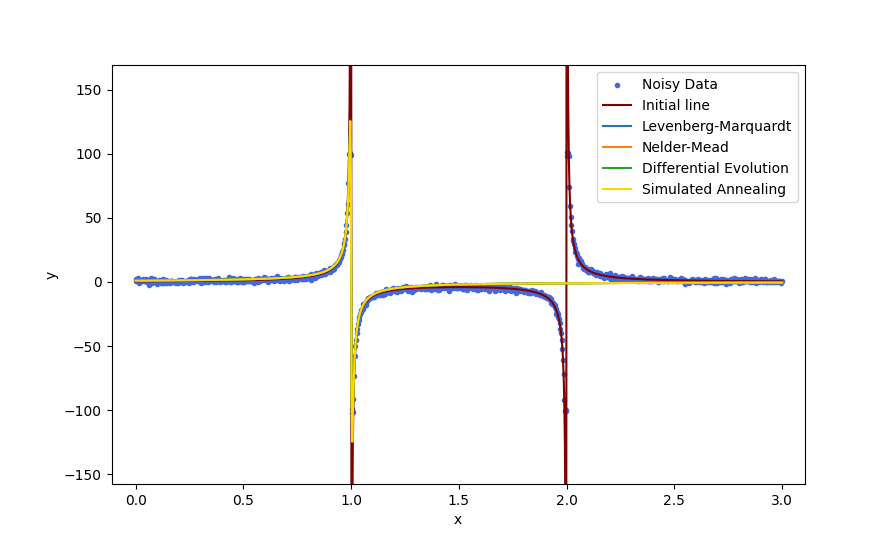
\includegraphics[width=\textwidth]{pic1.png}
\caption{Results of applying Nelder-Mead, Levenberg-Marquardt, Differential Evolution and Simulated Annealing to solve the problem of non-linear approximation.}
\end{figure}

\newpage

\textbf{Task 2.} Then, Simulated Annealing was used to solve the Travelling Salesman Problem on a dataset of 45 points on a plane (\href{https://github.com/Dormant512/itmo_lab_listings/blob/main/coords.txt}{.txt file with coordinates}). First, random initial path was chosen.

\vspace{-3mm}
\begin{figure}[!h]
\centering
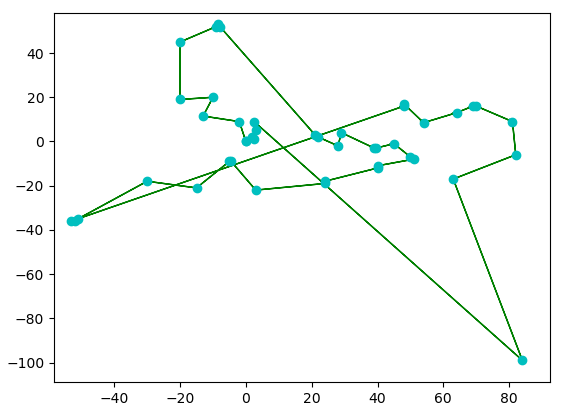
\includegraphics[width=0.6\textwidth]{pic2.png}
\caption{Initial path in Travelling Salesman Problem.}
\end{figure}

Then the path was optimized in a way that in each iteration cities were reconnected with a certain probability which depends on how optimal the new solution is and on the current temperature (the higher the temperature, the higher the probability of a jump). The resulting path is presented below:

\begin{figure}[!h]
\centering
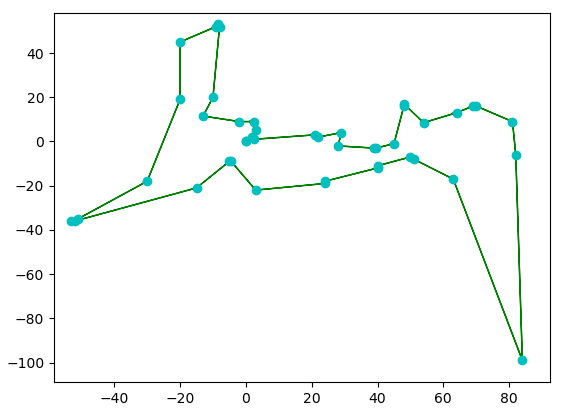
\includegraphics[width=0.6\textwidth]{pic3.png}
\caption{Optimized path in Travelling Salesman Problem.}
\end{figure}

The initial path was of length 732.6 units, while the optimized one is 621.0 units long. Optimizing the path was a big improvement, and the path seems quite optimal (judging visually). It is quite typical for metaheuristic algorithms to produce suboptimal solutions in short amounts of time, so the path may be not the absolute best.

\section*{Conclusions}
\addcontentsline{toc}{section}{Conclusions}

Metaheuristic methods such as Differential Evolution and Simulated Annealing were applied to the task of unconstrained nonlinear optimization, tested against each other, Nelder-Mead and Levenberg-Marquardt methods and compared in terms of perfomance.

\newpage

\section*{Appendix}
\addcontentsline{toc}{section}{Appendix}

GitHub link (task 1): \url{https://github.com/Dormant512/itmo_lab_listings/blob/main/lab4_1.py}.

GitHub link (task 2): \url{https://github.com/Dormant512/itmo_lab_listings/blob/main/lab4_2.py}.

\begin{figure}[!h]
\centering

\includegraphics[width=0.3\textwidth]{lab4-1.png}

\includegraphics[width=0.3\textwidth]{lab4-2.png}
\end{figure}


\end{document}
